\documentclass{pkuthesis}
\newcommand{\preTitleCn}{\zihao{2}}
\newcommand{\preTitleEn}{\zihao{3}}
\newcommand{\titleCn}{奖励塑造的困境破局:基于多选题的强化学习推理研究}
\newcommand{\titleEn}{Reward Shaping Breakthrough:  Enhancing RL Reasoning through Multi-Choice Paradigms}
\newcommand{\studentName}{王昱琛}
\newcommand{\studentID}{2100013153}
\newcommand{\schoolName}{北京大学}
\newcommand{\majorIn}{智能科学与技术}
\newcommand{\tutorName}{冯岩松}
\newcommand{\abstractCn}{随着大语言模型(LLM)在自然语言处理领域的迅猛发展,其在法律推理任务中的应用引起了广泛关注。然而,法律多选题因答案非唯一、推理链条复杂,对模型能力提出更高要求。本文提出了一种融合监督微调(SFT)与组相对策略优化(GRPO)的双阶段训练框架,在中国国家司法考试多选题(JEC-QA)案例分析子集上进行了验证。首先,利用 DeepSeek-R1 生成的长链思维示例对 Qwen-7B-Instruct 模型进行蒸馏并执行全量 SFT,以实现法律知识的冷启动;随后,基于格式奖励与严格准确性奖励,通过 GRPO 对模型进行强化学习微调,并引入 Dr. GRPO 长度偏差修正策略以抑制无效长尾推理。实验证明,本方法在测试集上将精确匹配率提升至 0.57,进一步的定量分析与结构化响应评估显示,模型在层次化段落组织、语篇连贯性和法条引用准确性等方面均有显著改进。}
\newcommand{\keywordsCn}{大语言模型;法律推理;监督微调;组相对策略优化(GRPO);JEC-QA;多选题
}
\newcommand{\abstractEn}{With the rapid advancement of large language models (LLMs), their application to legal reasoning tasks has garnered significant interest. However, multiple-choice legal questions present unique challenges due to non-unique correct answers and complex multi-step reasoning. This paper introduces a two-stage training framework combining Supervised Fine-Tuning (SFT) and Group Relative Policy Optimization (GRPO) on the case-analysis subset of the JEC-QA dataset. First, we distill chain-of-thought examples generated by DeepSeek-R1 into Qwen-7B-Instruct and perform full SFT for legal knowledge cold-start. Next, we fine-tune via GRPO using format and strict accuracy rewards, incorporating Dr. GRPO length-bias correction to mitigate inefficient long-tail reasoning. Experiments show our method achieves a mean\@1 accuracy of 0.57 on the test set. Quantitative evaluation and structured response analysis further demonstrate significant enhancements in hierarchical paragraph structuring, discourse coherence, and precise legal provision citation.
}
\newcommand{\keywordsEn}{Large Language Models; Legal Reasoning; Supervised Fine-Tuning; Group Relative Policy Optimization (GRPO); JEC-QA; Multiple-Choice Questions}
\usepackage[style=gb7714-2015]{biblatex}
\usepackage{amsmath}
\usepackage{amssymb}
\addbibresource{ref.bib}
\begin{document}

\section{引言}

\subsection{研究背景}

随着人工智能技术的快速发展,大语言模型(Large Language Models, LLMs)在自然语言处理任务中展现出卓越的性能,尤其在逻辑推理、语义理解和文本生成等方面取得了显著成果。然而,法律领域因其高度的专业性与复杂性,对模型推理能力提出了更高要求。法律问题通常具有非唯一性的特点,涉及多层次的法律逻辑与价值判断,这使得传统强化学习方法在法律任务中的应用面临诸多挑战。目前,主流的大语言模型推理能力多来源于数学与编程领域的训练,而本研究则创新性地探讨通过法律复杂问题训练,促进模型跨领域推理能力的提升。

已有研究表明,传统强化学习方法在面对答案唯一、评价标准明确的任务中表现良好;但在涉及多种合理解释的法律问题中,奖励函数的设计变得尤为困难。具体挑战包括:(1)法律问题的开放性导致标准化的评价指标难以确立;(2)合理答案可能基于不同的法律分析路径或表述方式;(3)法律推理过程通常要求严密的逻辑链条与专业知识支撑。因此,构建有效的法律推理模型,并通过强化学习技术优化其推理路径,成为当前亟需解决的重要科学问题。

近期研究显示,强化学习方法有助于提升大语言模型的推理能力。例如,DeepSeek-RL\cite{guo2025deepseek}、Qwen\cite{yang2024qwen2} 以及 Seed 系列模型\cite{seed2025seed} 表明,仅通过提供问题与答案对,模型可在缺乏显式推理监督的情况下,通过强化学习自主学习有效的推理策略。然而,这些方法在法律领域的适用性仍待验证,主要原因包括:(1)法律问题评估标准模糊,难以构建可通用的奖励函数;(2)缺乏标准化的评估机制,容易导致模型学习到偏离实际法律逻辑的策略。

为缓解上述问题,本研究选取不定项选择题(Multiple-Choice Questions, MCQs)作为训练数据的基础。该数据形式具有双重优势:一方面,MCQs提供了明确的选项空间,使基于规则的奖励函数设计更为可行;另一方面,多选题要求模型系统性地分析并评估所有选项,有助于培养其更全面的推理能力。本研究采用中国国家司法考试中的10,561道案例型多选题作为训练与评估语料,涵盖民法、刑法、诉讼法等主要法律门类,需具备专业级别的法律知识与推理能力。

\subsection{研究目标与贡献}

本研究旨在探索后训练(post-training)策略在法律领域的应用效果,重点关注如何通过强化学习优化大语言模型的法律推理能力。

具体研究目标如下:提升大语言模型在中国国家司法考试多项选择题中的答题准确率与推理质量,使模型能够在法律语境下自主学习并掌握系统的法律推理方法。

为实现上述目标,模型输入格式设计为:
\begin{quote}
“你是一名法学专家。现在请你解答司法考试中的一道选择题,请你找出所有正确的选项。每道题可能有一个或者多个正确答案。在解答之前,你需要先针对每个提供的选项给出详细的解释。你需要在回答的最后用大括号圈出给出的答案,例如 {B} 或者 {ABD}。”
\end{quote}

模型输出包括:
\begin{itemize}
\item “思考”部分:展现完整的法律推理链条;
\item “回答”部分:给出最终选项集合。
\end{itemize}

\subsection{论文结构}

本文采用系统化结构进行组织,各章节安排如下:

\begin{itemize}
\item 第二章为相关工作,系统梳理大语言模型中强化学习方法的研究进展及其在法律推理任务中的应用现状;

\item 第三章详细介绍本研究提出的方法,重点描述基于多选题的强化学习训练机制及其与监督微调的混合训练框架,包括奖励函数构建与训练策略设计;

\item 第四章构建实验框架,介绍后训练策略的具体实现,包括底层系统设计、基线模型选取及评估指标体系;

\item 第五章呈现实验结果与综合分析,通过定量指标与定性案例展示强化学习对模型推理能力的提升效果,并分析其背后机制;

\item 第六章为讨论部分,深入探讨本方法的优势与不足,提出改进方向并讨论方法在其他专业领域的潜在适用性;

\item 第七章总结全文,概括研究成果,并展望大语言模型在法律智能领域的未来发展趋势。

\end{itemize}

本研究不仅为法律智能提供了新的技术路径,其提出的混合训练范式与评估框架亦可推广至医疗诊断、金融分析等高专业性的人工智能应用领域。通过构建面向法律推理的大模型训练体系,我们希望推动人工智能向更强逻辑推理能力的方向迈进。

\section{相关工作}



近年来,强化学习(Reinforcement Learning, RL)被广泛应用于大语言模型(Large Language Models, LLMs)的微调与对齐过程中。其中,基于人类反馈的强化学习(Reinforcement Learning from Human Feedback, RLHF)成为主流技术框架,旨在训练奖励模型以捕捉人类偏好,并据此优化语言模型的输出策略。这类方法通常引入额外的奖励函数 $r_{\phi}(x, y)$ 对模型输出进行评分,并通过近端策略优化(PPO)\cite{schulman2017proximal}、直接偏好优化(DPO)\cite{rafailov2023direct} 等策略梯度算法对策略 $\pi_{\theta}(y \mid x)$ 进行更新,从而使模型输出更符合人类预期。这些技术的发展表明,强化学习能够在提升 LLM 可控性和对齐能力方面发挥重要作用。近期的研究也进一步指出,强化学习是引导 LLM 学习推理能力的关键途径。

LLM 的后训练(post-training)技术旨在在通用预训练模型基础上,结合领域数据和任务需求进一步提升模型性能,从而推动了如 DeepSeek-R1\cite{guo2025deepseek} 等大型后训练模型(Large-scale Re-trained Models, LRMs)的发展。这类策略主要包括:使用领域数据进行微调、结合 RLHF 实现人类偏好对齐,以及设计复杂的训练流程以增强模型的多步推理能力。这些方法共同构成了 LLM 从通用能力向领域能力演进的研究范式。

在法律推理智能化研究中,LLM 的应用已经进入纵深发展阶段,但距离司法实践的实际需求仍存在显著能力鸿沟。一方面,法律文本具有强逻辑性,要求模型具备多层级推理能力;另一方面,司法决策强调思维链条的可追溯性与可信度,呼唤模型的思考过程满足 TRACER 标准(Traceable, Reasonable, Accountable, Contextualized, Evidence-based, Rational)。为应对上述挑战,Lawyer LLaMA\cite{huang2023lawyer} 基于 LLaMA 对法律任务进行了微调,表现出对案件分析和法律推理的改进能力;ChatLaw\cite{cui2023chatlaw} 则结合法律知识检索、多专家融合和多智能体方法提升法律场景表现;LawGPT\cite{zhou2024lawgpt} 构建了高质量法律问答数据集,并在中文模型基础上进行了领域特定微调。然而,我们通过系统性分析发现,目前法律大模型普遍采用监督微调(Supervised Fine-Tuning, SFT)这一单一策略,在满足司法场景所需的知识完备性和推理可信度方面仍存显著差距。为此,我们提出融合 SFT 与 RLHF 的双阶段训练框架:首先通过法律数据的监督微调实现法理知识的冷启动,随后引入 RLHF 强化模型的推理能力与知识迁移能力。该混合式训练策略不仅加深模型对法律知识的内化,还显著提升了模型对法条与案例的动态匹配与推理能力,从而提高司法决策的合理性与可解释性。

自 DeepSeek 团队提出 GRPO(Group Relative Policy Optimization)算法以来 \cite{shao2024deepseekmath},其在数学推理等任务中展现出显著性能,但也暴露出训练稳定性差、奖励噪声大等问题。为应对上述挑战,研究者提出了多种改进方法,包括 DAPO(Decoupled Clip and Dynamic Sampling Policy Optimization)\cite{yu2025dapo} 和 Dr. GRPO\cite{liu2025understanding},进一步推动了 RL 算法的发展。

GRPO 的核心机制是通过分组估计(group estimation)方式计算优势函数,从而在无需 critic 模型的情况下降低计算资源消耗,同时保持模型训练的稳定性与高效性。其目标函数为:
\begin{equation}
\text{Objective} = \sum_{i} \sum_{t} \left( \frac{\pi(a_t|s_t)}{\pi_{\text{old}}(a_t|s_t)} \right)^{\text{clip}} A(s_t, a_t)
\end{equation}
其中优势函数 \( A(s_t, a_t) \) 计算方式为:
\begin{equation}
A(s_t, a_t) = r(s_t, a_t) + \gamma V(s_{t+1}) - V(s_t)
\end{equation}

在 GRPO 基础上,DAPO 和 Dr. GRPO 引入如下优化策略:
\begin{itemize}
    \item \textbf{删除 KL 约束}:提升模型自由度,突破参考模型性能上限 \cite{yu2025dapo}。
    \item \textbf{Clip-Higher 策略}:缓解熵崩塌,提高生成多样性 \cite{yu2025dapo}。
    \item \textbf{Token-Level Loss 调整}:增强模型对长文本的处理能力 \cite{yu2025dapo}。
    \item \textbf{难度偏差修正}:移除标准差归一处理,提升指标稳定性 \cite{liu2025understanding}。
    \item \textbf{动态采样机制}:过滤奖励全 0/1 样本,防止梯度停滞 \cite{yu2025dapo}。
    \item \textbf{超长奖励重构}:通过软性惩罚机制规避响应冗长问题 \cite{yu2025dapo}。
\end{itemize}

GRPO 系列算法在长文本生成中展现出显著提升,其优化方法为强化学习在语言生成任务中的进一步应用提供了新路径。

\subsection{推理能力与泛化性}

除了 DeepSeek-R1 中提出的 “AHA 时刻”外,强化学习还被发现能在训练过程中自然诱导模型产生自我验证、反思式推理等能力 \cite{el2025competitive}。这类能力在没有明确监督信号的情况下自发出现,表明 RL 具备促进认知过程发展的潜力。

尽管大部分 RL 推理研究集中于数学与代码领域,但已有工作证明 RL 能促进模型向其他结构化或非结构化领域的泛化。例如,Logic-RL\cite{xie2025logic} 通过规则驱动的训练,在逻辑谜题任务中取得成功,并在数学推理任务中迁移表现良好,验证了 RL 能独立于领域知识诱导通用推理机制。

更令人关注的是,一些推理模型(如 DeepSeek-R1\cite{guo2025deepseek})已将推理能力拓展至医学、化学、心理学等人文学科,结合生成式软评分机制处理非结构化答案,为构建跨领域通用推理模型奠定基础。下一步的研究方向包括将此类模型与工具调用、检索增强生成(RAG)等系统集成,OpenAI 最新发布的 o3 模型正朝这一方向迈进。

\subsection{数据集:JEC-QA 案例分析题}

本研究使用中国国家司法考试官方题库中的 JEC-QA 数据集\cite{zhong2020jec},该数据集广泛应用于法律人工智能领域,具有较高的权威性与代表性。

\begin{itemize}
\item \textbf{数据来源}:采自中国国家司法考试历年真题,涵盖民法、刑法、行政法、诉讼法等多个法律分支,具有良好的覆盖性与实用性。

\item \textbf{规模与结构}:
\begin{itemize}
\item 数据集中共包含 26,365 道多项选择题;
\item 每道题可能包含一个或多个正确答案;
\item 题型分为两类:\textbf{知识型问题}(注重法条记忆)与 \textbf{案例分析问题}(侧重法律推理)。
\end{itemize}

\item \textbf{研究子集选择}:本研究聚焦于其中 10,561 道 \textbf{案例分析问题},该题型通常涉及具体案情描述,要求应试者结合法律规范进行多步推理与判断,充分体现法律推理过程的复杂性。选择该子集的原因在于其更贴近真实法律实践,对模型的法律理解与推理能力提出更高要求。

\item \textbf{数据划分方式}:按照 8:2 的比例将案例分析题划分为训练集与测试集,分别包含 8,449 道与 2,112 道题目,确保训练与评估的均衡性与代表性。

\item \textbf{任务定义}:模型需完成以下三个关键步骤:
\begin{itemize}
\item 准确识别案情中的法律争议点;
\item 正确定位并引用适用的法律条文;
\item 通过多步法律逻辑推理,选出所有正确选项。
\end{itemize}
\end{itemize}

该任务对语言模型的逻辑推理能力、法理理解能力以及语言表达一致性提出了系统性挑战,适合作为评估模型法律智能表现的标准基准。

\section{方法}

\subsection{任务定义}
本研究旨在提升大型语言模型在中国国家司法考试多项选择题上的法律推理能力与答题准确率。具体定义如下:

\begin{itemize}
  \item \textbf{研究目标:}
    提升 LLM 在中国国家司法考试多选题上的法律推理质量及选项预测准确率。
  \item \textbf{输入:}
    法律多选题,包括案例描述与若干备选答案;模型需先对每个选项进行推理分析。
  \item \textbf{输出:}
    \begin{enumerate}
      \item \emph{思考(Reasoning)}:完整的法律推理链条,对各选项给出详细解释;
      \item \emph{回答(Answer)}:最终以大括号形式给出正确选项集合,如“\{B\}”或“\{ABD\}”。
    \end{enumerate}
\end{itemize}



\subsection{基于人类偏好的强化学习(RLHF)流程}
我们采用标准的基于人类反馈的强化学习(Reinforcement Learning from Human Feedback, RLHF)方法,对预训练语言模型进行微调。该流程包含以下关键步骤:
\begin{enumerate}
    \item \textbf{奖励模型训练}:利用人工标注的偏好数据,训练奖励模型 \( r_{\phi}(x, y) \)。该模型基于输入提示 \( x \) 和回答 \( y \),对样本对 \((x, y_1, y_2)\) 的质量进行评估。
    \item \textbf{策略优化}:在奖励模型的指导下,通过策略梯度方法优化语言模型策略 \( \pi_{\theta}(y \mid x) \),以提升其生成高质量回答的能力。
\end{enumerate}
由于司法考试题目对逻辑一致性和推理链条完整性的要求极高,RLHF 能有效引导模型生成更符合人类偏好的结构化解释。

\subsection{近端策略优化(PPO)}
PPO \cite{schulman2017proximal}是一种广泛应用于语言模型强化学习微调的 Actor-Critic 算法。PPO 通过联合训练一个值函数网络(Critic),并引入裁剪代理目标来限制策略更新的幅度,从而提高训练的稳定性和样本效率。其核心思想是通过裁剪重要性采样比率,确保策略更新不会偏离当前策略过远。

\text{PPO 方法}
PPO 是一种基于策略梯度的算法,结合值函数和广义优势估计(Generalized Advantage Estimation, GAE)来计算优势函数 \( \hat{A}_t \),并在奖励中加入 KL 散度惩罚项以稳定训练。其优化目标定义为:
\[
L^{\text{PPO}}(\theta) = \mathbb{E}_{(x, y) \sim D_{\pi_{\text{ref}}}} \left[ r_{\text{model}}(x, y) - \beta \, \text{KL}(\pi_{\theta}(y \mid x) \| \pi_{\text{ref}}(y \mid x)) \right]
\]
其中,\( r_{\text{model}}(x, y) \) 是奖励模型对生成结果 \( y \) 的评分,\( \pi_{\text{ref}} \) 为参考策略(通常为监督微调后的预训练模型),\( \beta \) 为 KL 惩罚系数。策略更新采用裁剪代理目标函数:
\[
L^{\text{CLIP}}(\theta) = \hat{\mathbb{E}}_t \left[ \min \left( r_t(\theta) \hat{A}_t, \, \text{clip}(r_t(\theta), \, 1 - \epsilon, \, 1 + \epsilon) \hat{A}_t \right) \right]
\]
其中,\( r_t(\theta) = \frac{\pi_{\theta}(a_t \mid s_t)}{\pi_{\theta_{\text{old}}}(a_t \mid s_t)} \) 表示当前策略与旧策略在时刻 \( t \) 的概率比,\( \hat{A}_t \) 为 GAE 估计的优势值。然而,PPO 在大规模语言模型中面临两大挑战:一是需要额外训练值函数网络以计算 GAE,增加了参数规模和训练成本;二是文本生成任务中通常仅在序列末尾获得回报信号,导致中间状态的价值估计困难,影响训练的稳定性与效率。为了解决 PPO 在 LM 中需训练 Critic 以及仅末尾奖励的问题,我们引入组相对策略优化(GRPO)方法,该方法以采样组为单位进行相对评价,无需 Critic 结构,且更加稳定高效。

\subsection{组相对策略优化(GRPO)}
GRPO \cite{shao2024deepseekmath}是一种无需值函数的策略优化算法,通过模型自身生成的多组回答样本进行相对评分,估计优势函数(Advantage Function)并更新策略。其主要特点包括:
\begin{enumerate}
    \item \textbf{无需值函数模型}:传统 PPO 依赖值函数 \( V(x) \) 估计优势,而 GRPO 基于策略采样的相对信息,通过组内奖励归一化估计优势,消除了对价值函数的依赖。
    \item \textbf{样本组评分机制}:对于输入 \( x \),从当前策略 \( \pi_{\theta} \) 生成多个回答 \( \{y_1, \dots, y_K\} \),并由奖励模型评分:
    \[
    r_i = r_{\phi}(x, y_i), \quad i = 1, \dots, K
    \]
    根据评分排序,为每个样本分配排名权重 \( \alpha_i \)(如 Softmax 归一化得分),用于构造相对优势。
    \item \textbf{优势函数估计}:
    \[
    A(x, y_i) = \alpha_i - \frac{1}{K} \sum_{j=1}^K \alpha_j
    \]
    其中,\( \alpha_i \) 可为 Softmax 输出或单调映射的排名指标。
    \item \textbf{策略更新目标}:
    GRPO 使用裁剪策略目标限制偏移:
    \[
    L^{\text{GRPO}}(\theta) = \hat{\mathbb{E}}_{(x, y_i) \sim \pi_{\theta_{\text{old}}}} \left[ \min \left( r_{\theta}(x, y_i) A(x, y_i), \, \text{clip}(r_{\theta}(x, y_i), \, 1 - \epsilon, \, 1 + \epsilon) A(x, y_i) \right) \right]
    \]
    其中,\( r_{\theta}(x, y) = \frac{\pi_{\theta}(y \mid x)}{\pi_{\theta_{\text{old}}}(y \mid x)} \)。
\end{enumerate}

\textbf{GRPO 方法}:  
\begin{figure}[h]
    \centering
    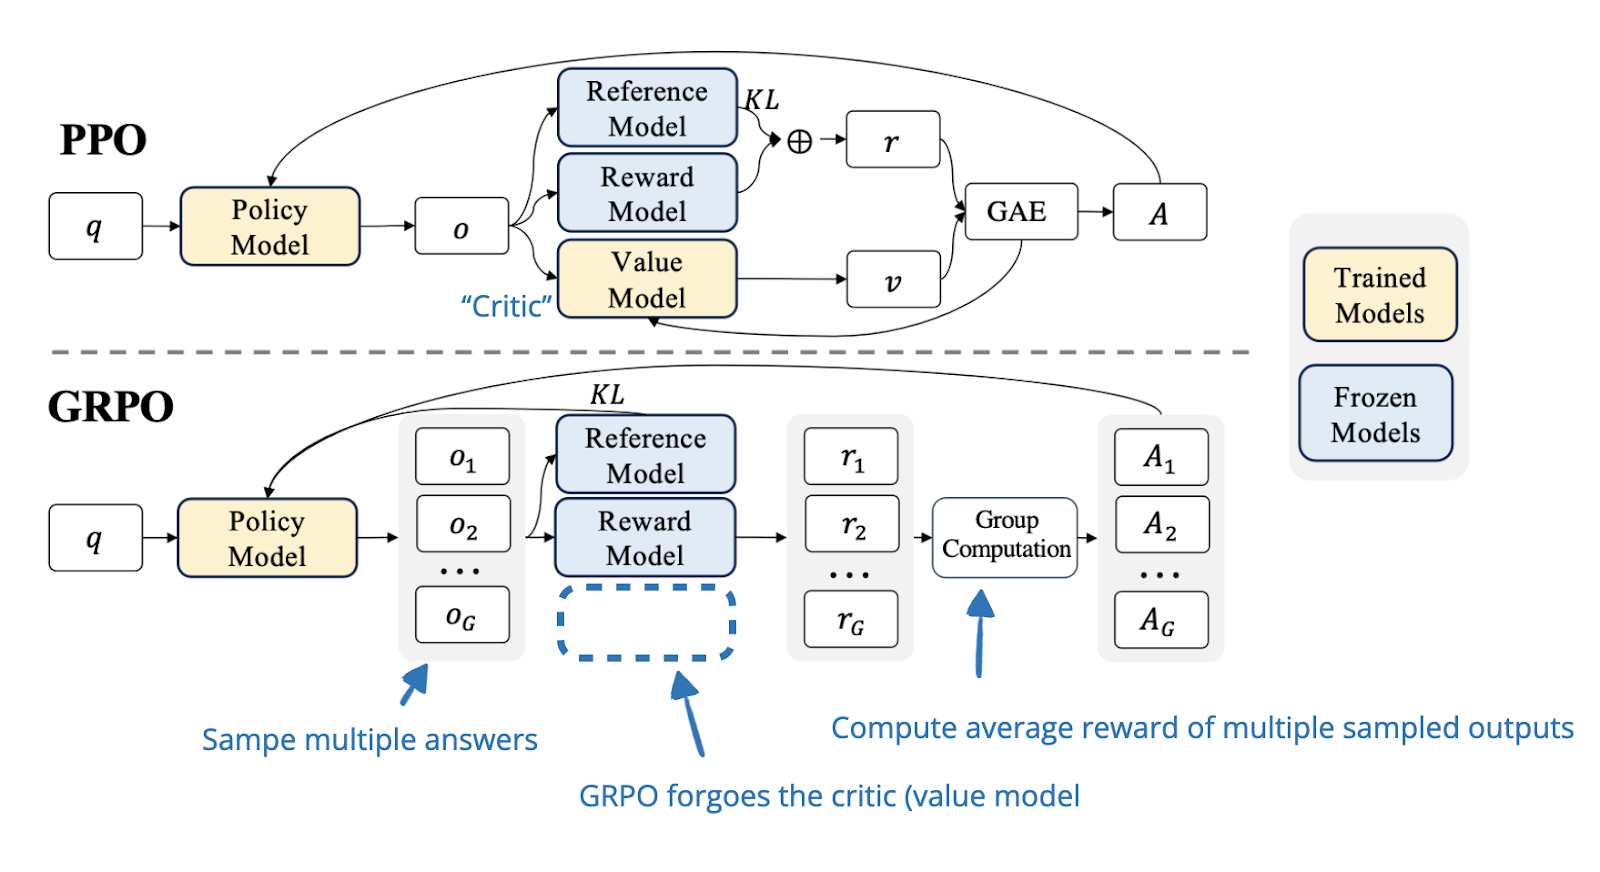
\includegraphics[width=1\textwidth]{figures/grpo.png}
    \caption{GRPO 方法示意图\cite{shao2024deepseekmath}}
    \label{fig:grpo}
\end{figure}
GRPO 通过对输入 \( x \) 生成 \( K \) 个回答 \( \{y_1, y_2, \dots, y_K\} \),利用奖励模型评分 \( r_i = r_{\phi}(x, y_i) \),并应用 Softmax 函数:
\[
\alpha_i = \frac{\exp(r_i / \tau)}{\sum_{j=1}^K \exp(r_j / \tau)}
\]
其中 \( \tau \) 为温度参数。相对优势定义为:
\[
A(x, y_i) = \alpha_i - \frac{1}{K} \sum_{j=1}^K \alpha_j
\]
高于均值的回答获得正优势,反之则为负优势。GRPO 通过组内比较直接评估优势,无需值函数网络,降低了内存和计算开销。


\subsection{DAPO 算法}
为提升模型在长链推理(Chain-of-Thought, CoT)任务中的表现,有工作引入了\textbf{解耦裁剪与动态采样策略优化(Decoupled Clipped and Dynamic Sampling Policy Optimization, DAPO)}算法\cite{yu2025dapo}。该算法通过一系列创新策略,优化了模型在复杂推理任务中的训练效率和性能。以下是其核心创新点的详细描述:

\begin{itemize}
    \item \textbf{解耦裁剪策略}:
    DAPO 采用非对称裁剪机制,分别设置下限 \( \varepsilon_{\text{low}} = 0.2 \) 和上限 \( \varepsilon_{\text{high}} = 0.28 \)。在传统的 PPO-clip 算法中,裁剪参数 \(\varepsilon\) 是对称的,即上下限相同,这限制了低概率动作(exploration token)的提升空间。DAPO 通过解耦上下裁剪参数,允许低概率动作的提升幅度更大,从而促进模型的多样性。具体而言,对于策略更新的裁剪目标函数 \(L^{CLIP}\),DAPO 定义为:
    \[
    L^{CLIP} = \mathbb{E}_{t} \left[ \min \left( \frac{\pi(a_t|s_t)}{\pi_{\text{old}}(a_t|s_t)} A^{\pi_{\text{old}}}(s_t, a_t), \; \varepsilon_{\text{high}} \right) - \max \left( \frac{\pi(a_t|s_t)}{\pi_{\text{old}}(a_t|s_t)} A^{\pi_{\text{old}}}(s_t, a_t), \; -\varepsilon_{\text{low}} \right) \right]
    \]
    其中,\(\pi(a_t|s_t)\) 是当前策略,\(\pi_{\text{old}}(a_t|s_t)\) 是旧策略,\(A^{\pi_{\text{old}}}(s_t, a_t)\) 是优势函数。这种非对称裁剪机制能够有效避免熵崩溃现象,同时提升模型的探索能力。

    \item \textbf{动态样本重采样}:
    DAPO 通过过采样并筛选出准确率非 0 或 1 的样本,确保每个样本都能提供有效的梯度信息。在传统的采样方法中,组内全对或全错的样本会导致优势函数为零,从而没有梯度,影响训练效率。DAPO 的动态采样策略通过过滤这些极端样本,确保每个采样组内的优势函数均非零。具体而言,对于采样组 \(G\),DAPO 仅保留满足 \(0 < \text{accuracy}(G) < 1\) 的样本组,从而提高训练效率并降低梯度方差。

    \item \textbf{Token 级策略梯度损失}:
    DAPO 在所有 token 上计算损失,赋予长序列更大的权重。传统的样本级损失计算方式(sample-level loss)对长回答和短回答赋予相同的权重,这在长链推理任务中是不合理的。DAPO 采用 token 级损失计算方式,定义为:
    \[
    L^{TOKEN} = \sum_{t=1}^{T} \log \pi(a_t|s_t) \cdot A^{\pi_{\text{old}}}(s_t, a_t)
    \]
    其中,\(T\) 是序列长度。通过这种方式,DAPO 对长回答中的高质量和低质量响应模式赋予更大的权重,从而提升模型在复杂推理任务中的表现。

    \item \textbf{过长奖励整形}:
    DAPO 采用软长度惩罚机制,其奖励函数定义为:
    \[
    R_{\text{length}}(y) = \begin{cases} 
    0, & |y| \leq L_{\text{max}} - L_{\text{cache}} \\ 
    \frac{(L_{\text{max}} - L_{\text{cache}}) - |y|}{L_{\text{cache}}}, & L_{\text{max}} - L_{\text{cache}} < |y| \leq L_{\text{max}} \\ 
    -1, & L_{\text{max}} < |y|
    \end{cases}
    \]
    其中,\(L_{\text{max}} = 16384\) 是最大允许长度,\(L_{\text{cache}} = 4096\) 是缓存长度。这种软惩罚机制能够有效惩罚过长的回答,同时避免因长度限制而引入的噪声。具体而言,当回答长度 \(|y|\) 超过 \(L_{\text{max}} - L_{\text{cache}}\) 时,奖励函数逐渐减小,直至达到最大长度 \(L_{\text{max}}\) 时,奖励值为 \(-1\)。这种机制能够引导模型生成更合理的回答长度,同时避免因长度限制而带来的梯度消失问题。
\end{itemize}


\subsection{Dr.GRPO 算法}
\textbf{Dr.GRPO 算法}\cite{liu2025understanding}是对 GRPO 的改进,通过修正偏见提升推理能力。其主要改进包括:
\begin{itemize}
    \item \textbf{去除响应长度偏见}:移除除以响应长度的项,确保策略更新不受长度影响。
    \item \textbf{消除问题难度偏见}:移除组内奖励标准差归一化,使学习过程更平衡。
    \item \textbf{调整基线计算}:优化基线估计为:
    \[
    \mathbb{E}[r_k] = \frac{1}{K} \sum_{k=1}^K r_k
    \]
\end{itemize}
目标函数为:
\[
J_{\text{Dr.GRPO}}(\theta) = \mathbb{E}_{\{\tau_k\}_{k=1}^K \sim \pi_{\theta_{\text{old}}}}\left[\sum_{k=1}^{K} \sum_{t=1}^{|o_k|} \hat{\rho}_{k,t}(\theta) (r_k - \mathbb{E}[r_k])\right]
\]

\subsection{方法小结}
我们首先定义了多选题法律推理任务的输入输出格式,并采用 RLHF 框架提升生成质量。随后,我们从经典的 PPO \cite{schulman2017proximal}出发,分析其在法律推理任务中的局限,引入无需 Critic 的 GRPO 方法\cite{shao2024deepseekmath}提升训练效率。最后,我们进一步介绍了 DAPO \cite{yu2025dapo},Dr.GRPO \cite{liu2025understanding}等GRPO的改进算法,以提升模型在长链推理任务中的表现。


\subsection{奖励函数}
\textbf{格式奖励}

格式奖励的核心目标是实施指导模型推理过程的结构性约束,以确保其响应遵守特定的逻辑框架。具体来说,我们要求模型的输出包括以下结构:\texttt{<思考>} 标签和 \texttt{<回答>} 标签,它们在解决问题时明确概述了模型所采取的推理路径\cite{guo2025deepseek}。例如,这可能涉及在法律问题中确定有争议的观点,召回相关的法规或判例法,并比较不同的法律概念。

\textbf{准确性奖励}

单项选择问题在2或4个选项中有一个正确的答案。通常可以通过不完整或表面的推理来解决它们,因为有限的答案空间使模型可以在不完全理解基本概念的情况下获得正确的答案。这种局限性使此类格式在训练强大的推理能力方面的有效性降低了,尤其是在法律等复杂领域。相比之下,具有一个或多个正确答案的多选题问题要求该模型可以全面评估每个选项的正确性,而没有猜测或部分推理的空间。
我们设计了一个严格的奖励机制,仅当模型在所有其他情况下都可以选择所有正确的选项并分配零奖励(奖励$=0$)时,才能提供积极的反馈(奖励$=1$)。令 $S_{\text{true}}$ 为多选题问题的正确选项集合,$S_{\text{pred}}$ 为模型预测的选项集合。则准确性奖励 $R_{\text{accuracy}}$ 定义为:
$$ R_{\text{accuracy}}(S_{\text{pred}}, S_{\text{true}}) = \begin{cases} 1 & \text{if } S_{\text{pred}} = S_{\text{true}} \\ 0 & \text{otherwise} \end{cases} $$
它确保正确的选项与准确和完整的推理过程相关联。这种严格的奖励机制消除了在强化学习过程中基于捷径的解决方案的可能性,并迫使该模型对当前的任务有了更深入的了解。


\section{实验框架}


\subsection{基线模型(Baselines)}

\begin{itemize}
\item \textbf{Qwen2.5-7B-Instruct}:作为当前中文领域表现最强的开源语言模型之一\cite{yang2024qwen2},该模型被用于评估法律任务上的 zero-shot 能力,作为原始模型性能参考。

\item \textbf{R1 蒸馏模型}:我们基于 Qwen2.5-7B-Instruct 的响应(R1)结果构建蒸馏数据,对 student 模型进行监督训练。该做法受到近年来在数学和编程任务中取得显著成效的 teacher-student 蒸馏范式启发\cite{guo2025deepseek},作为监督蒸馏方法的基线。

\end{itemize}

\subsection{监督微调(SFT)阶段}

我们采用 LLaMA-Factory 和 DeepSpeed 作为监督微调的训练框架。LLaMA-Factory 是一个专为大型语言模型开发的高效训练工具,支持全参数微调、LoRA 适配、多 GPU 并行训练等功能\cite{llamafactory},在本研究中用于组织模型微调流程。

在蒸馏实验设置中,我们首先基于 \texttt{jec-qa-1-multi-choice} 数据集,使用 DeepSeek-R1 模型生成的回答作为 teacher signal 构建蒸馏语料。随后,利用该语料对 Qwen-7B-Instruct 模型进行全量监督微调。训练采用如下超参数设置:训练轮次为 2 epoch,batch size 为 32,最大上下文长度为 4096,学习率设为 $1 \times 10^{-5}$,使用余弦退火调度器(cosine decay schedule),并在前 10\% 的训练步骤中进行预热(warm-up)。该设置基于任务复杂度与模型容量的经验选择,旨在提升训练收敛性与稳定性。

\subsection{GRPO 阶段}

在监督微调后,我们进一步对微调后的 Qwen-7B-Instruct 模型执行 GRPO(Group Relative Policy Optimization)训练。该阶段的奖励函数结合了两项指标:

\begin{itemize}
\item \textbf{准确性奖励(Accuracy Reward)}:根据模型输出与标准答案的匹配度计算;
\item \textbf{格式奖励(Format Reward)}:鼓励模型输出结构规范、答案格式统一的响应。
\end{itemize}

通过设计多维奖励信号,引导模型在生成过程中兼顾法律结论的正确性与答案呈现的一致性,从而更好地适应实际应用需求。

\subsection{训练加速框架:DeepSpeed 与 ZeRO 策略}

我们使用 DeepSpeed 作为底层训练加速器。DeepSpeed 是微软推出的分布式训练库,核心为 ZeRO(Zero Redundancy Optimizer)优化策略。ZeRO 通过将模型训练过程中的优化器状态、梯度以及模型参数在多张 GPU 之间分布切分,大幅降低了单卡显存需求,并提升了训练效率。其分为三个阶段:

\begin{itemize}
\item \textbf{Stage 1}:优化器状态分区;
\item \textbf{Stage 2}:在 Stage 1 基础上进一步对梯度分区;
\item \textbf{Stage 3}:进一步将模型参数分区,实现最大程度的内存优化,适用于超大规模模型的训练。
\end{itemize}

该方案使得我们能够在有限的硬件资源条件下,对 7B 参数级别模型进行高效训练与优化。




\subsection{VeRL}
除了模型训练框架,推理阶段的高效引擎也是研究热点。vLLM是一个面向LLM推理的高吞吐量库,采用分页注意力(Paged Attention)等技术来优化GPU内存管理。实验结果表明,与传统的HuggingFace Transformers和OpenAI TGI等框架相比,vLLM在相同硬件资源下可实现数倍以上的吞吐量提升,同时大幅减少KV缓存浪费。vLLM支持多种主流模型架构(如LLaMA、Mistral、Qwen、DeepSeek等),并提供量化与工具调用等扩展功能。这些优化使得在法律等领域部署大型LLM时,推理效率和可扩展性得到显著提高。
\textbf{General Concepts}\\
\textbf{RL}: 强化学习(Reinforcement Learning,RL)在近年来因 \texttt{o1/r1} 等技术突破而成为大模型训练的热门方向。VeRL 是一款面向 RL 的高效训练框架。从自然语言处理(NLP)的视角来看,RL 与传统的监督微调(SFT)主要有以下差异:
\begin{enumerate}
    \item \textbf{引入惩罚信号}:SFT 仅模仿正例,而 RL 同时对优质样本给予奖励、对劣质样本施加惩罚。无论策略梯度、GRPO、Reinforce 还是 PPO,本质上都在设计奖励/惩罚的颗粒度(token / macro action / sequence 等)与强度(是否使用 baseline、KL 约束、clip 等)。
    \item \textbf{允许模型自采样并在线训练自身}:SFT 通常依赖人工标注或其他模型生成的数据(蒸馏)。RL 则可实时采样并利用当前策略更新模型。
\end{enumerate}

\paragraph{on‐policy vs.\ online}
\begin{itemize}
    \item \textbf{online}: 当前策略能否与环境交互并实时获取奖励信号(如数学题求解后立即得知正确与否)。在 GUI Agent、自动驾驶等场景需构建复杂模拟器。
    \item \textbf{on‐policy}: 训练数据是否由最新策略采样。在实践中常预采大量经验数据再分 mini‐batch 更新,除首个 mini‐batch 外均为 off‐policy。
\end{itemize}
常用的 GRPO/Reinforce/PPO 等方法一定是 \emph{online},但不必然 \emph{on‐policy}(取决于 mini‐batch 数)。

\paragraph{Ray 系统概览}
Ray 是一套分布式计算框架,为 VeRL 和 OpenRLHF 等 RL 框架提供 Actor 角色管理及资源调度。核心概念如下:
\begin{itemize}
    \item \textbf{Ray Actor}: 有状态远程任务(由 \texttt{ray.remote} 装饰的 Python 类),运行时对应独立进程(勿与 RL 中的"Actor"角色混淆)。
    \item \textbf{Ray Task}: 无状态远程任务(由 \texttt{ray.remote} 装饰的函数),局部变量对提交方不可见,可视作无状态。
    \item \textbf{资源管理}: Ray 可按 CPU/GPU/内存等进行自动调度,也支持 \textit{placement group} 将 Actor 固定在同一或不同设备 bundle 上。
    \item \textbf{异步执行}: Ray 调度默认异步,任务提交即返回对象引用;用户可用 \texttt{ray.get}/\texttt{ray.wait} 阻塞或轮询结果。
\end{itemize}
在 RL 训练中引入异步设计,可让 Actor/Critic/Generator/RM 等角色的计算流水重叠,例如在 Actor 更新上一批数据时,Generator 已可并行生成下一批样本。鉴于 o1‐style RL 的主要瓶颈位于 rollout,未来的优化方向是更充分地异步化 rollout(如夜间充分利用线上推理集群空闲算力)。

\paragraph{并行策略}
\begin{itemize}
    \item \textbf{3D 并行}: LLM 训练(megatron‐lm)与推理引擎(vllm、sglang)已广泛支持数据并行(DP)、张量并行(TP)与流水线并行(PP)。VeRL 新版本基于 Ulysses 进一步支持序列并行(SP),对长文本 RL 尤为关键。
    \item 不同角色在不同阶段可灵活调整 3D 并行组合,VeRL 借助 \emph{hybrid engine} 做了诸多优化,如零冗余参数 re‐sharding。
\end{itemize}

\paragraph{FSDP 与 Megatron}
FSDP(Meta 提出)与 Megatron 分别代表两套分布式训练框架:
\begin{itemize}
    \item \textbf{FSDP}: 将模型参数(权重、优化器状态等)在 GPU 间分片存储,仅按需通信,并重叠计算与通信,逻辑清晰、易支持新结构,研究友好。
    \item \textbf{Megatron}: 在百亿级模型训练中更具性能优势,参数 re‐sharding 开销低,工程友好。
\end{itemize}
VeRL 同时兼容两套引擎。

\subsubsection{VeRL‐related Concepts}

\paragraph{Hybrid Flow}
RL 训练逻辑涉及多模型交互。VeRL 将数据流抽象为两层:
\begin{itemize}
    \item \textbf{控制流}: 高层描述角色间交互,如 Actor 生成经验后,Critic/RM/Reference 计算得分,然后计算 GAE 与损失。
    \item \textbf{计算流}: 低层描述单角色内的前向‐反向、优化器更新、自回归生成等。
\end{itemize}

\paragraph{Single Controller vs.\ Multiple Controllers}
\begin{itemize}
    \item \textbf{Single Controller}: 单中心控制器统一管理所有子模块,架构清晰、易维护。VeRL 采用该模式实现 RL 算法控制流,极大便利新算法开发。
    \item \textbf{Multiple Controllers}: 将控制逻辑分散到多控制器,通过集合通信同步,通信开销低但逻辑更复杂。VeRL 在\emph{计算流}维度使用此模式,以降低通信负载。
\end{itemize}
VeRL 通过多层级 Worker(\texttt{RayWorkerGroup} $\rightarrow$ \texttt{WorkerDict} $\rightarrow$ \texttt{ModelWorker} $\rightarrow$ \texttt{ParallelWorker})封装计算流。

\paragraph{Hybrid Engine — 模型放置策略}
\begin{enumerate}
    \item \textbf{分开放置}: 角色独立占用设备,可异步执行但 GPU 利用率略低。
    \item \textbf{分组放置}: 将角色分组共置,既能重叠执行又减少空闲:
    \begin{itemize}
        \item 典型分组:Actor/Generator 同组(需实时同步参数),Critic/RM 与 Reference 分别单独。
    \end{itemize}
    \item \textbf{全部共置}: 所有角色共用设备,GPU 始终被占用,但只能串行。
\end{enumerate}
VeRL 通过 \texttt{resource pool} 灵活支持以上策略,并设计 \texttt{worker\_dict} 以动态角色切换(\texttt{reload/offload params})。

\paragraph{数据传输协议}
为适配不同角色的数据切分需求,VeRL 设计了统一的数据分发(Dispatch)与收集(Collect)协议,并以 Python 装饰器形式绑定到 Worker 方法,实现透明的数据流与执行模式。

\paragraph{训练流程示意}
\begin{enumerate}
    \item \texttt{RayPPOTrainer} 向 \texttt{RayWorkerGroup} 发送方法调用。
    \item \texttt{RayWorkerGroup} 先执行数据分发,再根据执行模式决定哪些 Worker 执行任务。
    \item 结果经收集逻辑处理后返回 Trainer。
\end{enumerate}

\subsubsection{RL 设置}
本研究的 RL 阶段采用 VeRL(Sheng et al., 2024)实现组相对策略优化(GRPO)。以下结合 VeRL 的特性,阐述 GRPO 实现步骤。

\paragraph{1.\ 初始化与核心组件}
GRPO 训练由 \texttt{GRPOTrainer} 管理,初始化需配置:
\begin{itemize}
    \item \textbf{策略模型(Actor)}: 采用 QWEN2.5‐7B‐Instruct。
    \item \textbf{参照模型(Reference)}: 同架构 SFT 模型,用于计算 KL 惩罚。
    \item \textbf{奖励函数}: 采用基于规则的格式与准确性奖励,无需外部 RM。
\end{itemize}

\paragraph{2.\ Rollout 生成}
\begin{itemize}
    \item \textbf{权重同步}: 每轮大迭代开始,通过 \texttt{RolloutShardingManager} 将最新 Actor 权重同步到推理引擎(vLLM/SGLang)。
    \item \textbf{提示采样}: 从数据集中抽取一批 prompt,由 \texttt{generate\_sequences} 调用推理引擎生成响应。
    \item \textbf{多样生成}: 配置 \texttt{actor\_rollout\_ref.rollout.n}(本研究设 $K{=}7$)并设置 \texttt{temperature=1.0},为每个 prompt 并行生成 $K$ 条不同响应。
    \item \textbf{奖励计算}: 对每条响应计算格式与准确性奖励 $r_i$(详见 \ref{subsection:reward_function})。
    \item \textbf{数据封装}: 保存 prompt、$K$ 条响应、token 级对数概率、mask 与奖励,组成后续训练批次;prompt 最长 512 token,响应最长 2048 token。
\end{itemize}

\paragraph{3.\ 对数概率计算}
\begin{itemize}
    \item \textbf{旧策略对数概率 $\text{old\_log\_prob}$}: 使用未更新的 Actor 对 (prompt, response) 再次前向传播获取。原因:\textit{(i)} 高性能推理引擎通常不保存完整 token‐level log‐prob;\textit{(ii)} 直接保存可能受数值波动与并行策略影响。
    \item \textbf{参照策略对数概率 $\text{ref\_log\_prob}$}: Reference Model 对同一批数据计算 log‐prob,用于 KL 约束。首轮迭代时与 \text{old\_log\_prob} 相同。
\end{itemize}

\paragraph{4.\ 奖励与优势估计}
\begin{itemize}
    \item \textbf{奖励整合}: VeRL 支持外部 RM 或自定义函数(本研究采用规则奖励)。
    \item \textbf{优势函数}: 调用 \texttt{compute\_advantage},依据 GRPO 公式(公式 \textit{Y})在组内(同一 prompt 的 $K$ 样本)计算相对优势,并可选择标准化 (\texttt{norm\_adv\_by\_std\_in\_grpo})。
\end{itemize}

\paragraph{5.\ 策略更新(Mini‐batch 内循环)}
对每个 mini‐batch 执行:
\begin{itemize}
    \item 计算新策略对数概率 $\text{new\_log\_prob}$。
    \item \textbf{策略梯度损失} $\text{pg\_loss}$:由 \texttt{compute\_policy\_loss} 依据公式 \textit{Z} 计算,含 cliprange 等裁剪。
    \item \textbf{熵正则}:鼓励探索。\texttt{entropy\_coeff} 控制权重。
    \item \textbf{KL 惩罚}:当前策略与 Reference 之间的 KL 散度,乘 \texttt{kl\_loss\_coef} 加入总损失。
    \item 反向传播并更新 Actor 参数。
\end{itemize}
完成全部 mini‐batch 后,同步最新权重,进入下一大迭代的经验收集。


\section{Metric评测}
由于每个多选题示例都有一个或多个答案,因此我们评估了实例和选项级别的性能。给定的答案 $y^{(i)}_{\text{pred}}$ 和地面真相 $y^{(i)}_{\text{gold}}$ 对于第 $i$ 个问题,两个指标表示如下:

\textbf{精确匹配}:这衡量了预测答案与正确答案完全匹配的实例的比例。
$$ \text{精确匹配} = \frac{1}{N} \sum_{i=1}^{N} \mathbf{1}(y^{(i)}_{\text{pred}} = y^{(i)}_{\text{gold}}) $$
其中 $\mathbf{1}(\cdot)$ 是指示函数,如果内部的条件为true,则等于1,否则为0。它评估模型是否可以为问题提供完全正确的答案。对于多选题,这意味着预测的选项集合与真实的选项集合完全一致。

\textbf{召回和精确度}:我们根据模型对单个答案选项的预测来计算召回和精度得分。
令 $N$ 为问题总数。对于第 $i$ 个问题,令 $P_i$ 为模型预测的正确选项集合,$G_i$ 为实际的正确选项集合。
则选项级别的精确度 (Precision) 和召回率 (Recall) 定义为:
$$ \text{Precision}_{\text{option}} = \frac{\sum_{i=1}^N |P_i \cap G_i|}{\sum_{i=1}^N |P_i|} $$
$$ \text{Recall}_{\text{option}} = \frac{\sum_{i=1}^N |P_i \cap G_i|}{\sum_{i=1}^N |G_i|} $$
其中 $|S|$ 表示集合 $S$ 的基数。如果某个问题模型没有预测任何选项(即 $|P_i|=0$),则该问题对精确度的分子和分母的贡献均为0。
通常也会计算 F1 分数:
$$ F1_{\text{option}} = 2 \cdot \frac{\text{Precision}_{\text{option}} \cdot \text{Recall}_{\text{option}}}{\text{Precision}_{\text{option}} + \text{Recall}_{\text{option}}} $$


\section{实验思路与尝试}

本节介绍我们围绕多选法律推理任务所开展的一系列研究,包括奖励函数设计、蒸馏模型的强化学习改进,以及基于结构化分析的案例研究。

\subsection{Zero-RL(无 SFT)}

\textbf{基础模型:}Qwen-2.5-7B-Instruct。  
\textbf{训练流程:}直接对预训练模型应用多种强化学习算法(GRPO / Dr. GRPO)。  
\textbf{实验目的:}验证在无监督微调条件下,强化学习是否本身即可提升模型的法律推理能力。

\subsection{SFT + RL(蒸馏冷启动)}

\textbf{蒸馏数据:}使用 DeepSeek-R1 在 JEC-QA 多选案例上的思维链响应(Long COT SFT)。  
\textbf{SFT阶段:}
\begin{itemize}
  \item 模型:Qwen-2.5-7B-Instruct
  \item 训练配置:2 个 epoch,batch size = 32,context length = 4096,学习率 $1\times10^{-5}$,使用 cosine 退火调度并加上 10\% warm-up。
\end{itemize}

\textbf{RL阶段:}在经过 SFT 的模型上应用 GRPO 进行强化学习,奖励函数包括格式奖励(Format Reward)和完全匹配准确性奖励(Exact Match Accuracy Reward)。

\subsection{奖励函数改进与长度控制}

我们进一步设计了更为细致的奖励机制:

\begin{itemize}
  \item \textbf{Hybrid Reward:}结合完全匹配与部分匹配以缓解严格匹配对模型探索能力的限制。
  \item \textbf{去除格式奖励:}在部分实验中去除格式奖励以分析其作用。
  \item \textbf{Cosine Penalty:}惩罚“无效长尾推理”,防止无效内容拉长响应。
  \item \textbf{Repetition Penalty:}抑制重复生成。
\end{itemize}

\begin{table}[h]
  \centering
  \caption{不同奖励类型定义及特点}
  \begin{tabular}{l|p{8cm}|c}
    \hline
    奖励类型 & 定义与说明 & 特点 \\
    \hline
    Exact Match & 若预测集合 $S_{\text{pred}}$ 与真实集合 $S_{\text{true}}$ 完全一致则奖励 1,否则为 0。 & 严格,限制探索 \\
    Partial Match & 对错误多选(FP)与漏选(FN)进行惩罚,公式见下文。 & 可调,平衡精确与召回 \\
    Format & 响应需包含“思考”与“回答”结构。 & 训练早期收敛快 \\
    \hline
  \end{tabular}
\end{table}

DeepSeek-R1 的研究指出,SFT 后接 RL 能带来额外性能增益。然而我们发现,直接对 DeepSeek-R1-Distill-Qwen-7B 应用 GRPO 会收敛缓慢,性能提升有限(mean@1 ≈ 0.214),主要原因在于:

\begin{itemize}
  \item 蒸馏数据域与实际任务存在偏差;
  \item 思维链提示存在冷启动问题;
  \item 缺乏 Instruct 微调导致模型对 Prompt 遵循性差。
\end{itemize}

为此,我们引入全量 SFT 冷启动以提升模型初始表现,并进一步配合 RL 优化。

\subsection{奖励函数构建与实验分析}

我们分别设计了以下两类准确性奖励函数:

\begin{enumerate}[label=(\arabic*)]
  \item \textbf{完全匹配奖励(Exact Match)}:
    \[
    R_{\mathrm{exact}}(S_{\mathrm{pred}}, S_{\mathrm{true}})
      = \begin{cases}
          1, & S_{\mathrm{pred}} = S_{\mathrm{true}},\\
          0, & \text{otherwise}.
        \end{cases}
    \]
  \item \textbf{部分匹配奖励(Partial Match)}:
    \[
    R_{\mathrm{partial}} = \max\left(0,\;1 - x \cdot (\mathrm{FP} + \mathrm{FN})\right),\quad x \ge 0.5
    \]
    其中 FP 表示多选错误数,FN 表示漏选错误数,$x$ 控制惩罚强度。
\end{enumerate}

\begin{figure}[h]
  \centering
  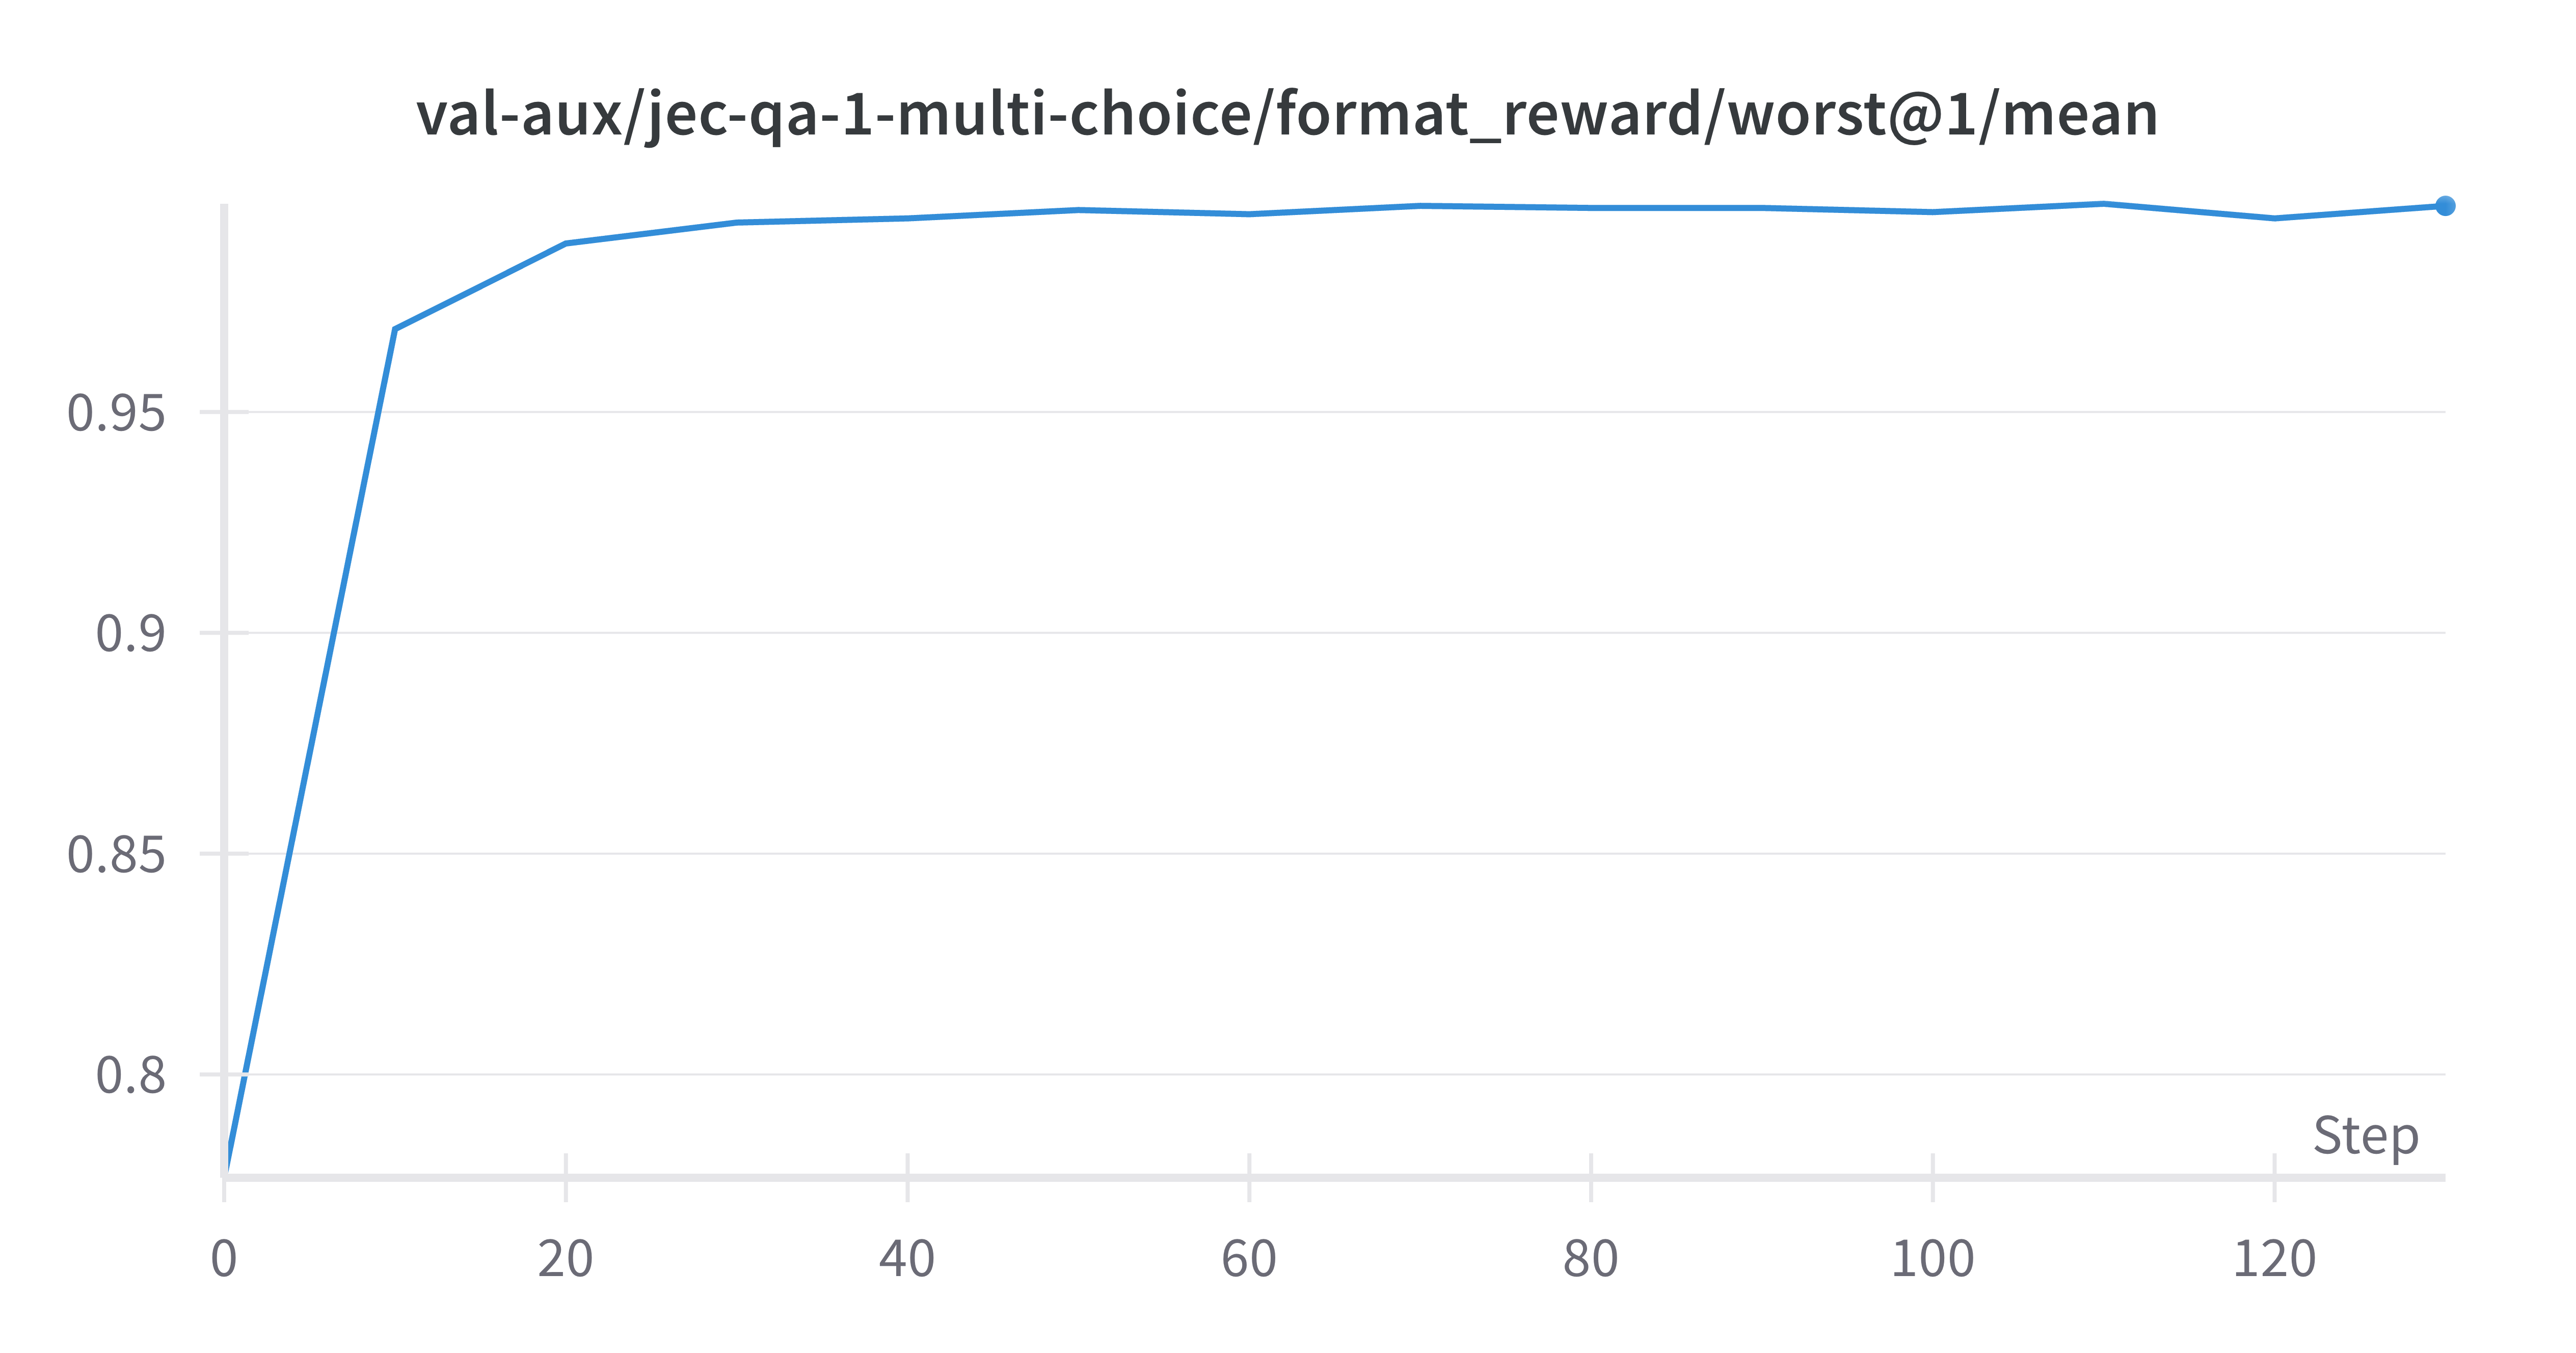
\includegraphics[width=0.8\textwidth]{figures/format.png}
  \caption{移除格式奖励后的准确率变化}
  \label{fig:format}
\end{figure}

\textbf{实验结果对比:}

\begin{table}[h]
  \centering
  \caption{不同惩罚系数 $x$ 下的性能表现}
  \begin{tabular}{l|c|c|c}
    \hline
    惩罚系数 $x$ & 精确匹配率(mean@1) & 召回率(worst@1) & 精确度(worst@1) \\
    \hline
    完全匹配 & 0.576 & 0.770 & 0.777 \\
    $x=0.7$  & 0.569 & 0.790 & 0.777 \\
    $x=0.9$  & 0.564 & 0.794 & 0.772 \\
    \hline
  \end{tabular}
\end{table}

\textbf{关键发现:}
\begin{itemize}
  \item 随着 $x$ 增大,召回率逐步上升但精确度略有下降;
  \item 当 $x = 0.7$ 时性能达成较好平衡;
  \item 完全匹配适合用于严格评估场景,但可能限制边缘样本的探索。
\end{itemize}

\textbf{最终采用的奖励组合为:}
\[
R = R_{\mathrm{format}} + R_{\mathrm{accuracy}},
\]
其中 $R_{\mathrm{accuracy}}$ 为根据实验设置切换的准确性奖励类型。

\subsection{蒸馏模型的强化学习改进}

我们参考 DeepSeek-R1 的策略,先在 JEC-QA 上蒸馏思维链响应,再进行 SFT 微调,随后使用 GRPO 强化学习。

\textbf{实验发现:}
\begin{itemize}
  \item 若直接对蒸馏模型进行 GRPO,训练收敛缓慢,mean@1 仅为 0.214;
  \item 采用全量 SFT 冷启动后,RL 性能显著提升;
  \item 结构性响应(编号段落、连接词、前置引导语等)比例显著提升,推理过程更具法律解释力。
\end{itemize}

\begin{figure}[h]
  \centering
  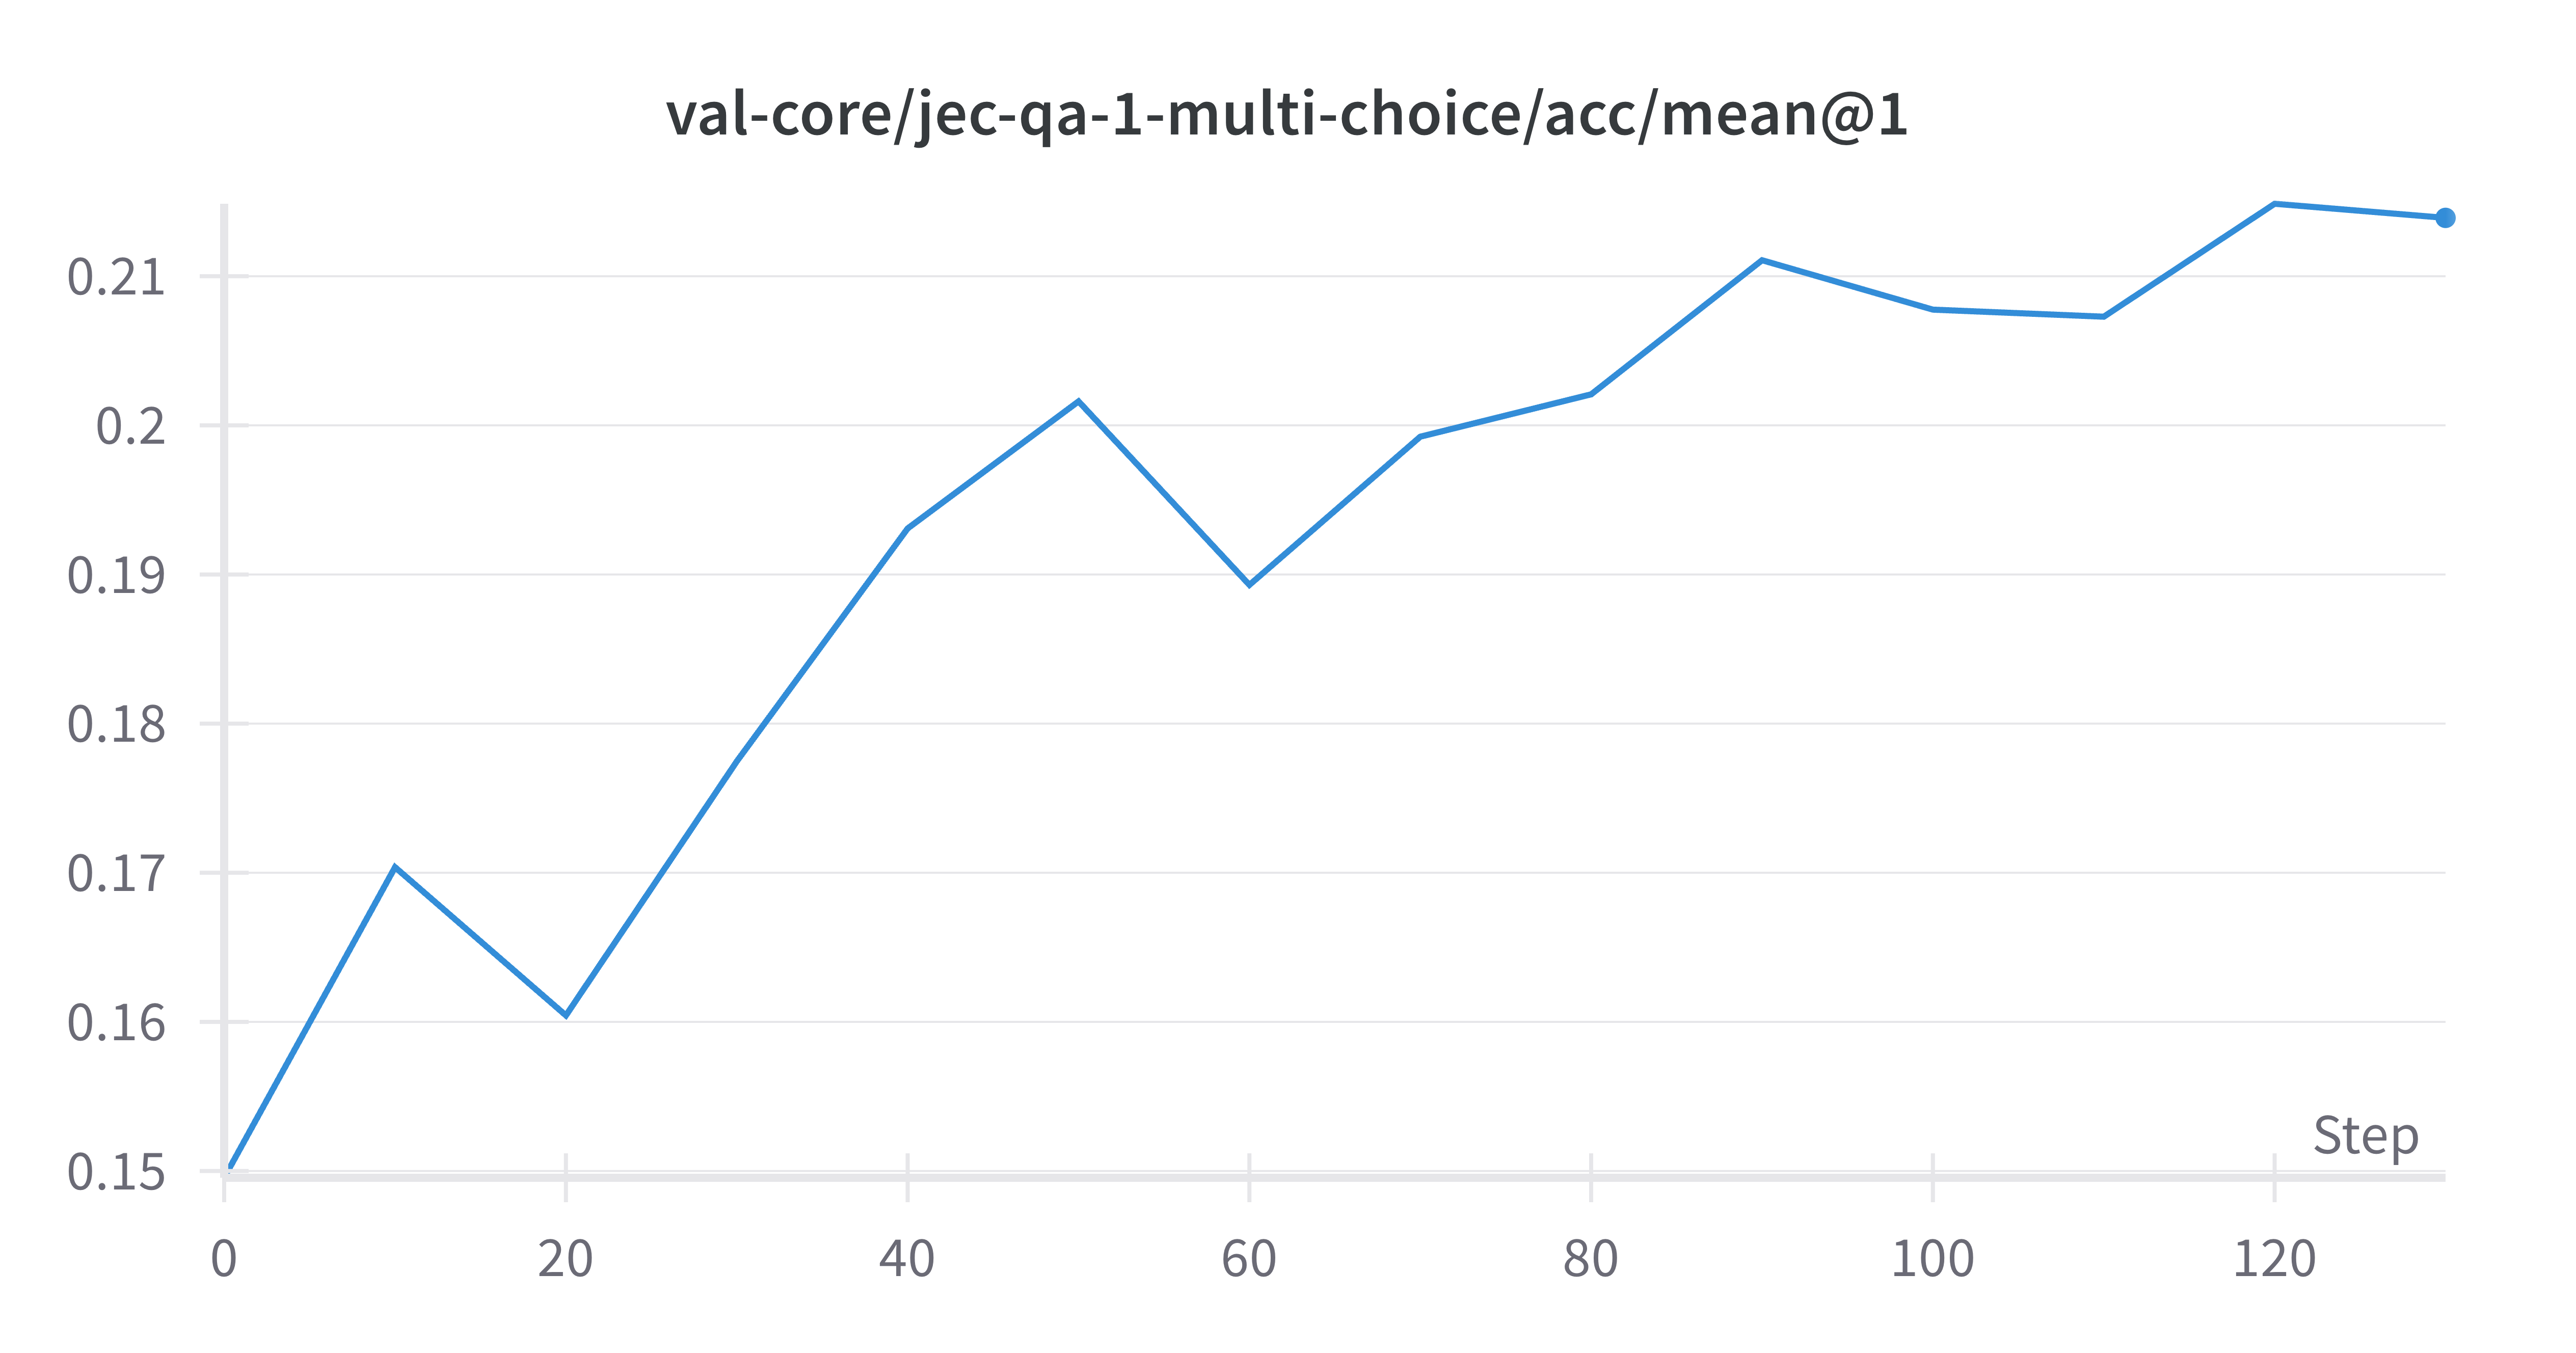
\includegraphics[width=0.8\textwidth]{figures/GRPO_DeepSeek-R1-Distill-Qwen-7B.png}
  \caption{DeepSeek-R1-Distill-Qwen-7B 在 GRPO 中的收敛曲线}
  \label{fig:grpo_distill}
\end{figure}

\subsection{全量 SFT 冷启动 + GRPO 训练}

\textbf{训练配置:}
\begin{itemize}
  \item \textbf{SFT阶段:}
    \begin{itemize}
      \item 2 个 epoch,batch size = 32,context length = 4096;
      \item 学习率 $1\times10^{-5}$,使用 cosine 退火调度与 10\% warm-up;
      \item 初始截断设为 1024 tokens,导致平均响应长度显著下降;
      \item 初始 clip ratio 达 0.6。
    \end{itemize}
  \item \textbf{GRPO阶段:}
    \begin{itemize}
      \item 奖励:格式奖励 + 完全匹配准确性奖励;
      \item Rollout 数 $K=7$,temperature = 1.0,clip range $\epsilon = 0.2$。
    \end{itemize}
\end{itemize}

\textbf{性能比较:}

\begin{table}[h]
  \centering
  \caption{不同训练阶段模型在验证集上的准确率(mean@1)}
  \label{tab:acc-distill-sft-grpo}
  \begin{tabular}{l|c}
    \hline
    模型阶段 & 准确率 (mean@1) \\
    \hline
    原版 DeepSeek-R1 & 67.4\% \\
    SFT 冷启动 & 42.4\% \\
    全量 SFT(2048 tokens) + GRPO & \textbf{53.2\%} \\
    \hline
  \end{tabular}
\end{table}

\begin{figure}[h]
  \centering
  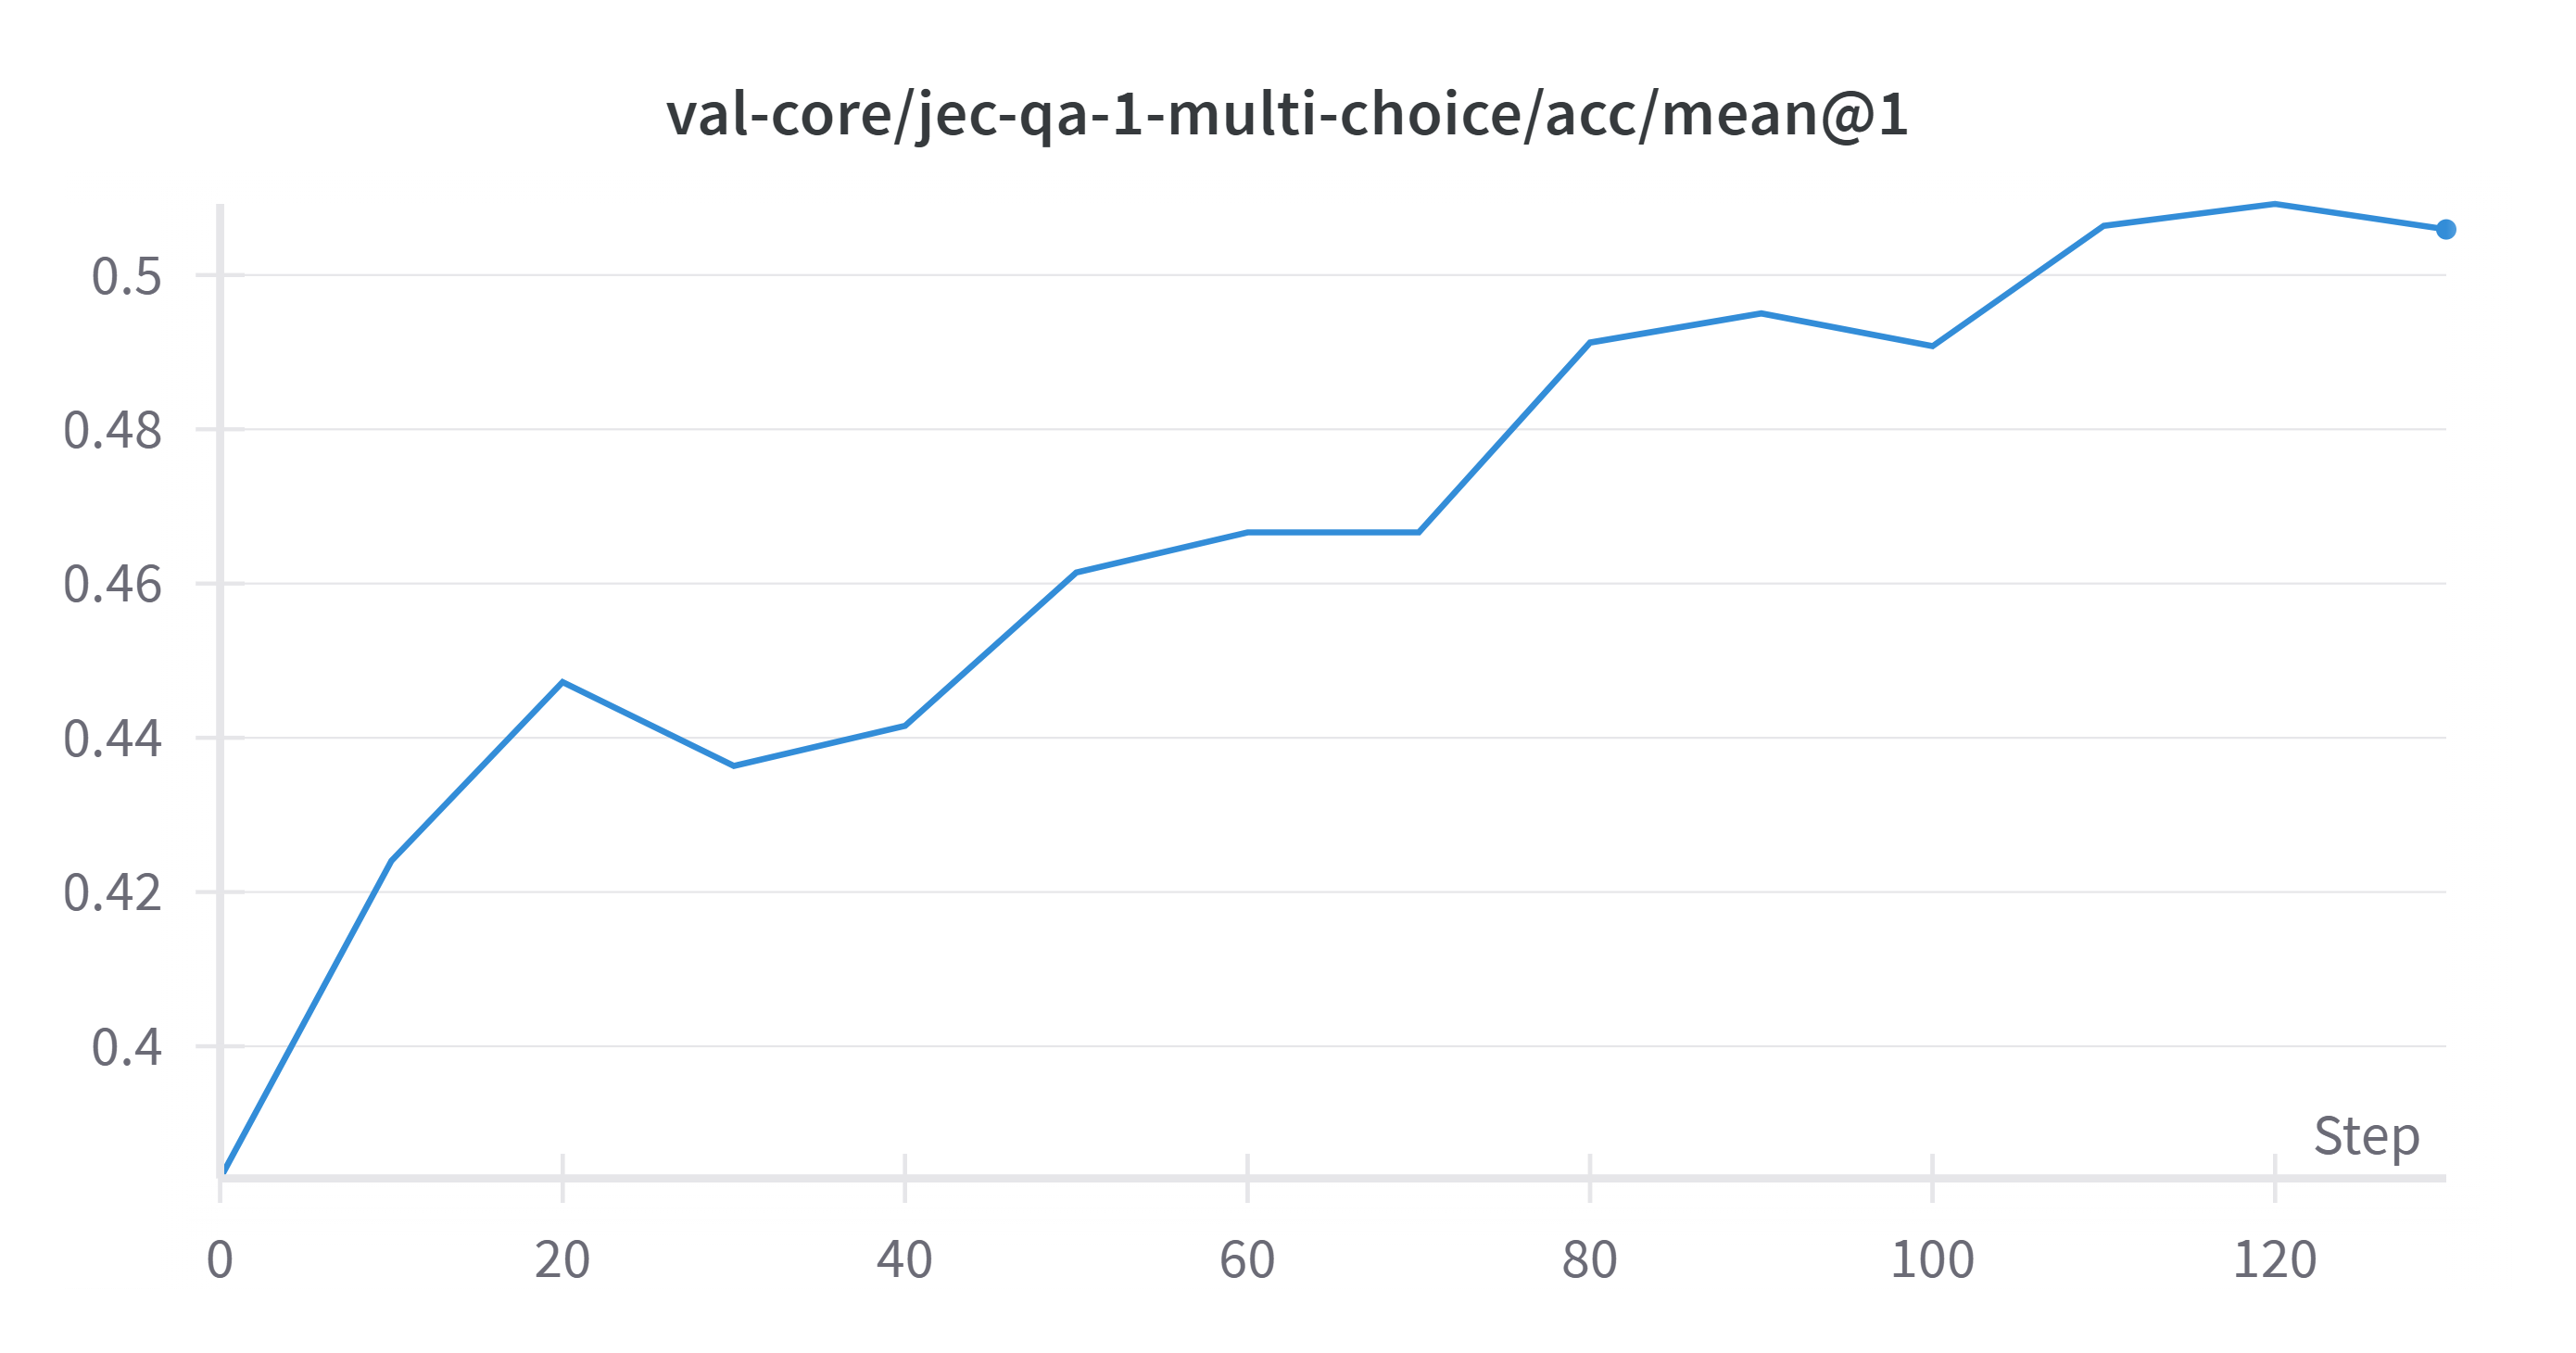
\includegraphics[width=0.8\textwidth]{figures/sft4096.png}
  \caption{SFT-4096 模型在 GRPO 强化学习过程中的准确率变化}
  \label{fig:acc-comparison}
\end{figure}

综上所述,虽然强化学习可显著提升模型在多选法律问答任务中的表现,但由于基础模型能力有限,其最终性能仍略低于强基础模型(如原版 DeepSeek-R1)。后续将考虑更强基础模型及多阶段微调策略,以进一步缩小差距。



\printbibliography
\end{document}
